% !TEX encoding = UTF-8
% !TEX TS-program = pdflatex
% !TEX root = ../tesi.tex

%**************************************************************
\chapter{Dataset e modello di machine learning}
\label{cap:machine-learning}
%**************************************************************

\intro{In questo capitolo si andrà a descrivere il dataset utilizzato, la sua elaborazione e lo sviluppo del modello di machine learning.}\\

%**************************************************************
\section{Descrizione del dataset}
\subsection{Descrizione del tipo di dati ricercati}
Dopo l'incontro con un esperto in geologia, a cui l'azienda si è rivolta per una consulenza, si è deciso di descrivere gli esempi che andranno in input al modello di machine learning attraverso la loro firma spettrale.
La firma spettrale è una caratteristica che ogni materiale ha, ed è specifica per ogni combinazione di riflessi e assorbimenti delle radiazioni elettromagnetiche (EM) a diverse lunghezze d'onda. Conoscendo la firma spettrale di un oggetto, è possibile identificarlo univocamente.
Un esempio di firma è quello riportato nella figura 2.1, presa dal dataset di seguito presentato.
\begin{figure}
    \centering
    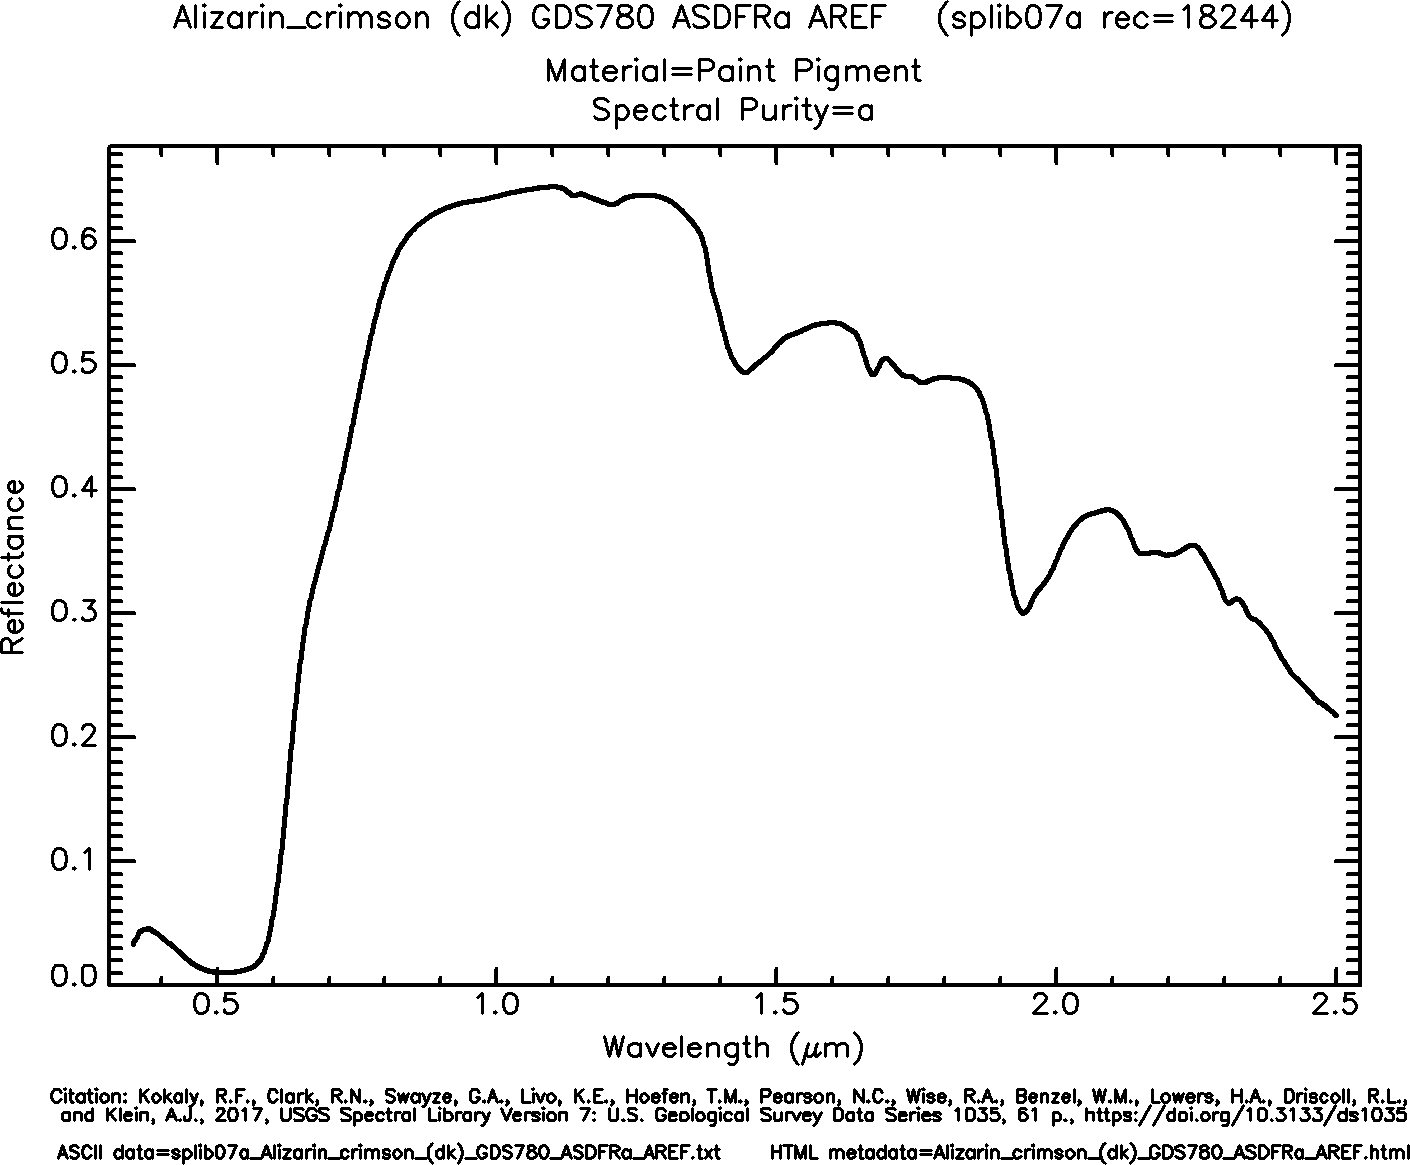
\includegraphics[width=0.8\textwidth]{esempio_firma.png}
    \caption{Firma spettrale dell'alizarina cremisi}
\end{figure}

\subsection{USGS Spectral Library}
Il dataset scelto per verificare la fattibilità della classificazione di oggetti tramite la loro firma spettrale è stato quello dello United States
Geological Survey, un'agenzia scientifica del governo degli Stati Uniti d'America.
Il dataset è denominato USGS Spectral Library Version 7.
Questo insieme di dati è stato raccolto nel corso degli anni dai ricercatori dell'ente menzionato facendo rilevazioni su migliaia di materiali in laboratorio,
usando diversi tipi di spettrometri, i quali coprono lunghezze d'onda che vanno dall'ultravioletto all'infrarosso (da \unit{0.2}{\micro\meter} a \unit{200}{\micro\meter}).
Gli strumenti usati, in dettaglio, sono:
\begin{itemize}
    \item Beckman\textsuperscript{TM} 5270, il quale copre l'intervallo spettrale dai 0.2 ai 3 \micro\meter;
    \item i modelli standard, high-resolution (hi-res) e high-resolution Next Generation (hi-resNG) della Analytical Spectral Devices (ASD);
          che coprono tutti dai 0.35 ai 2.5 \micro\meter;
    \item Nicolet\textsuperscript{TM} Fourier Transform Infra-Red (FTIR) che copre dai 1.12 ai 216 \micro\meter;
    \item NASA Airborne Visible/Infra-Red Imaging Spectrometer (AVIRIS) il quale copre dai 0.37 ai 2.5 \micro\meter.
\end{itemize}
Le classi di materiale prese in considerazione sono:
\begin{itemize}
    \item minerali;
    \item terreno (incluso rocce e minerali);
    \item rivestimenti su superfici rocciose;
    \item liquidi;
    \item composti organici;
    \item materiali artificiali;
    \item vegetazione e altri materiali biologici.
\end{itemize}
Una caratteristica degna di nota del dataset è che in corrispondenza di lunghezze d'onda il cui valore di riflettanza fosse stato eccessivamente sporcato da gas atmosferici questo è stato impostato a $-1.23 \cdot 10^{34}$, il quale corrisponde al "deleted channel" del software SPECPR (SPECtrum Processing Routines). Di conseguenza questi valori dovranno essere rimossi, per evitare che il modello prenda degli input inconsistenti durante il processo di allenamento.

\subsection{Elaborazione dei dati}
In primo luogo è stato necessario formattare i dati contenuti nel dataset in modo che fossero poi pronti come input per il modello di machine learning. Originariamente questi erano contenuti in file formato \verb|.txt| codificati in ASCII. In particolare erano suddivisi in cartelle in base allo spettrometro usato nelle rilevazioni e all'anno in cui sono state effettuate. Dentro ognuna di queste poi, vi era una cartella per ogni classe di materiale, contenente le lo spettro luminoso di ogni materiale. Il file con la lunghezza d'onda era comune per tutti i materiali. Per questa attività si sono realizzati degli script in linguaggio Python, i quali rimuovevano caratteri come spazi e stringhe. Il risultato, per ogni cartella, è un file \verb|data.txt| in cui ogni linea identifica una rilevazione. In particolare il primo numero intero $n \in \{ 0 .. 6 \}$ identifica la classe di appartenenza secondo questa mappa:
\begin{itemize}
    \item $0 \rightarrow$ materiali artificiali
    \item $1 \rightarrow$ rivestimenti
    \item $2 \rightarrow$ liquidi
    \item $3 \rightarrow$ rocce minerali
    \item $4 \rightarrow$ composti organici
    \item $5 \rightarrow$ terreno
    \item $6 \rightarrow$ vegetazione
\end{itemize}
Successivamente ci sono $k$ numeri che rappresentano lo spettro luminoso, seguiti da altrettanti per le lunghezze d'onda corrispondenti. Più in dettaglio, il numero n-esimo nell'array dello spettro luminoso corrisponde all'n-esimo nell'array delle lunghezze d'onda. Il valore $k$ dipende dallo strumento usato per la rilevazione.\\
Vista l'eterogeneità delle righe del file, le quali hanno lunghezze diverse a causa della diversità delle misurazioni effettuate, si è resa necessaria una fase di uniformazione. Questa è stata effettuata usando il software proprietario MATLAB\_R2021A, lo script è il seguente: